% Drawing 144/05-4 -- folder 144, batch 05, archive page 91 (PDF page 92).
% Transcription: petite sphère en marge : sur l'équateur $0$, $a_0$, $1$ ; derrière, $a_\infty$, $\infty$, $a_1$.
% Kind: small sphere with six points on the equator. Method 2 (schematic redraw from the facsimile). Status: ok.
% Notes: In front: 0, a_0, 1; behind: a_infty, infinity, a_1.
% Coordinates: 1 unit = 1 mm = 1/100 of the crop width (bbox in page fractions: [0.13, 0.27, 0.25, 0.34]).
% Redrawn by Claude (claude-opus-5-5), issue #73, 2026-11-07; not checked by a human; not compiled (no TeX in the session).
% Rights: reproduces part of the work -- behind RENDER_TRANSCRIPTS, never published by itself.
\documentclass[tikz,border=3pt]{standalone}
\usepackage{amsmath,amssymb}
\usetikzlibrary{patterns,arrows.meta}
\tikzset{pencil/.style={black!45}, struck/.style={black!35}, mark/.style={circle,draw,inner sep=1.3pt}, pt/.style={circle,fill,inner sep=0.9pt}, opt/.style={circle,draw,fill=white,inner sep=1.1pt}}
\begin{document}
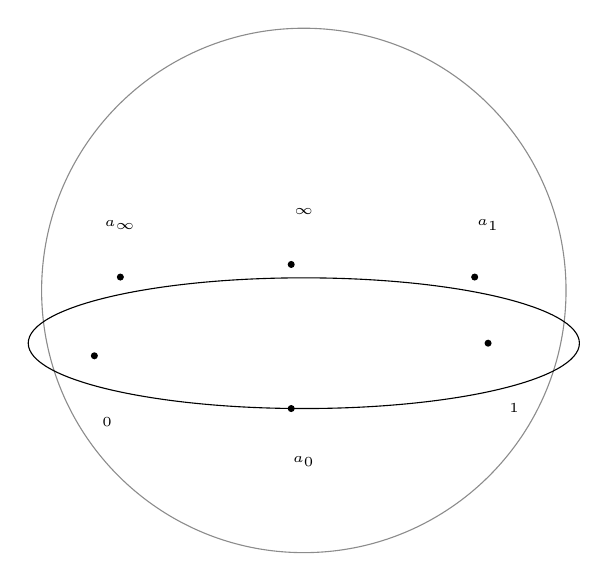
\begin{tikzpicture}[x=1mm,y=1mm,line cap=round,line join=round,font=\scriptsize]
\draw[pencil] (48.3,-41.2) circle[radius=33.3];
\draw (48.3,-47.9) ellipse[x radius=35, y radius=8.3];
\node[pt] at (21.7,-49.5) {};
\node[pt] at (46.7,-56.2) {};
\node[pt] at (71.7,-47.9) {};
\node[pt] at (25,-39.5) {};
\node[pt] at (46.7,-37.9) {};
\node[pt] at (70,-39.5) {};
\node[inner sep=1pt] at (23.3,-57.9) {\tiny $0$};
\node[inner sep=1pt] at (48.3,-62.9) {\tiny $a_0$};
\node[inner sep=1pt] at (75,-56.2) {\tiny $1$};
\node[inner sep=1pt] at (25,-32.9) {\tiny $a_\infty$};
\node[inner sep=1pt] at (48.3,-31.2) {\tiny $\infty$};
\node[inner sep=1pt] at (71.7,-32.9) {\tiny $a_1$};
\end{tikzpicture}
\end{document}
